\documentclass[compress]{beamer}
\usepackage{ifthen,verbatim}

\newcommand{\isnote}{}
\xdefinecolor{lightyellow}{rgb}{1.,1.,0.25}
\xdefinecolor{darkblue}{rgb}{0.1,0.1,0.7}

%% Uncomment this to get annotations
%% \def\notes{\addtocounter{page}{-1}
%%            \renewcommand{\isnote}{*}
%% 	   \beamertemplateshadingbackground{lightyellow}{white}
%%            \begin{frame}
%%            \frametitle{Notes for the previous page (page \insertpagenumber)}
%%            \itemize}
%% \def\endnotes{\enditemize
%% 	      \end{frame}
%%               \beamertemplateshadingbackground{white}{white}
%%               \renewcommand{\isnote}{}}

%% Uncomment this to not get annotations
\def\notes{\comment}
\def\endnotes{\endcomment}

\setbeamertemplate{navigation symbols}{}
\setbeamertemplate{headline}{\mbox{ } \hfill
\begin{minipage}{5.5 cm}
\vspace{-0.75 cm} \small
\end{minipage} \hfill
\begin{minipage}{4.5 cm}
\vspace{-0.75 cm} \small
\begin{flushright}
\ifthenelse{\equal{\insertpagenumber}{1}}{}{Jim Pivarski \hspace{0.2 cm} \insertpagenumber\isnote/\pageref{numpages}}
\end{flushright}
\end{minipage}\mbox{\hspace{0.2 cm}}\includegraphics[height=1 cm]{../cmslogo} \hspace{0.1 cm} \includegraphics[height=1 cm]{../tamulogo} \hspace{0.01 cm} \vspace{-1.05 cm}}

\newcommand{\s}[1]{{\mbox{\scriptsize #1}}}

\begin{document}
\begin{frame}
\vfill
\begin{center}
\textcolor{darkblue}{\Large Proposed Muon Alignment Constants Update}

\vfill
\begin{columns}
\column{0.6\linewidth}
\begin{center}
\large
Jim Pivarski on behalf of the

Muon Alignment Group
\end{center}
\end{columns}

\vfill
 9 August, 2010

\end{center}
\end{frame}

%% \begin{notes}
%% \item This is the annotated version of my talk.
%% \item If you want the version that I am presenting, download the one
%% labeled ``slides'' on Indico (or just ignore these yellow pages).
%% \item The annotated version is provided for extra detail and a written
%% record of comments that I intend to make orally.
%% \item Yellow notes refer to the content on the {\it previous} page.
%% \item All other slides are identical for the two versions.
%% \end{notes}

\small

\begin{frame}
\frametitle{Motivation}
\begin{itemize}
\item Because of the constants roll-back in May, we have been using a
  muon geometry with known imperfections:
\begin{itemize}
\item whole muon system is rotated 0.7~mrad around the beamline with
  respect to the tracker
\item endcap geometry is missing chamber corrections from
  photogrammetry (PG) and beam-halo
\end{itemize}
\end{itemize}

\vfill
\hspace{-0.83 cm} \textcolor{darkblue}{\Large Proposed update}

\begin{itemize}\setlength{\itemsep}{0.25 cm}
\item \textcolor{darkblue}{GlobalPositionRcd (whole muon system coordinate frame):} include
  the measurement derived from tracks (next page)
\item \textcolor{darkblue}{DTAlignmentRcd (barrel chamber, superlayer, and layer
  positions):} leave them as they are (hardware-derived), but note that
  track-based (TB) and hardware-derived (HW) results differ in
  systematically important ways (work in progress)
\item \textcolor{darkblue}{CSCAlignmentRcd (endcap chamber and layer positions):} use HW +
  beam-halo + PG update presented last time
\end{itemize}
\end{frame}

\begin{frame}
\frametitle{Global position}
\begin{itemize}
\item Connection of muon system coordinate frame to the tracker coordinate frame is difficult using HW-only measurements because some steps have mm-scale uncertainties
\item Using tracks, this connection is straight-forward and does not require large datasets
\item Alexander Spiridonov presented a robust method to determine the placement of a HW geometry with respect to the tracker

\href{http://indico.cern.ch/getFile.py/access?contribId=68&sessionId=9&resId=0&materialId=slides&confId=91797}{\tiny \textcolor{blue}{http://indico.cern.ch/getFile.py/access?contribId=68\&sessionId=9\&resId=0\&materialId=slides\&confId=91797}}

\item This is a full 6-DOF correction, but the parameter with the largest update is a 0.7~mrad rotation around the beamline
\begin{itemize}
\item chamber-by-chamber TB corrections show the same trend
\item the measured-but-not-applied HW correction also agrees
\end{itemize}

\item We use this for all TB-vs-HW studies in the rest of this talk,
  so that we study differences in the shape of the detector, not global offset

\item We propose to update the GlobalPositionRcd to this one, so that the HW geometry already in the DB will become correctly centered
\end{itemize}
\end{frame}

\begin{frame}
\frametitle{Barrel TB and HW geometries}

\begin{itemize}
\item Both methods have independently ``found'' the DT chambers at a
  level of at least a few mm in the sense that they are both
  substantial corrections relative to design and highly correlated with each other
\item This picture shows geometry differences in 3 DOF for TB-minus-HW, TB-minus-design, HW-minus-design (all wheel~0)
\end{itemize}

\vfill
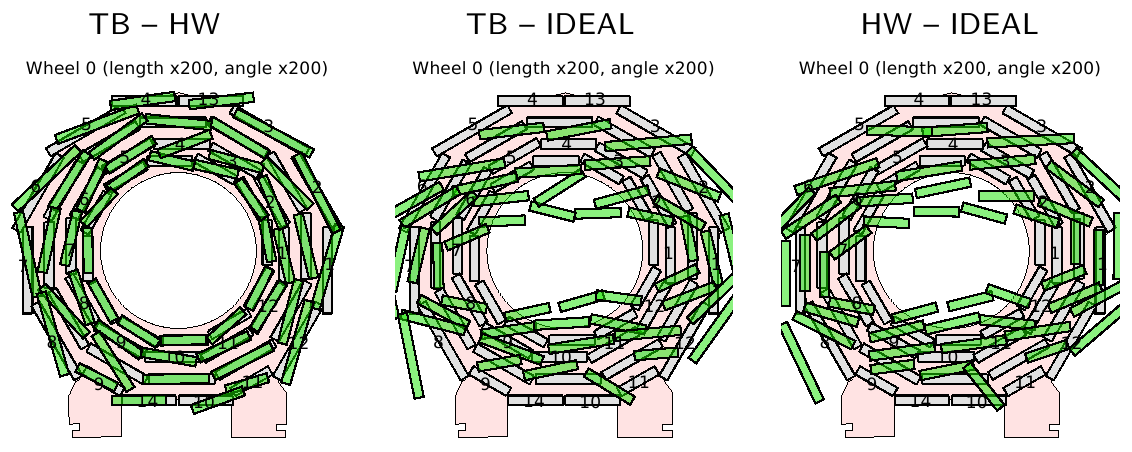
\includegraphics[width=\linewidth]{tb-hw_wheel0.png}

\mbox{\scriptsize {\bf N.B.} in this picture, displacements and angle differences have been exaggerated by 200$\times$\hspace{-1 cm}}
\end{frame}

\begin{frame}
\frametitle{Zero-field PG$-$HW test}
\hfill \begin{minipage}{0.75\linewidth}
\begin{itemize}
\item Before going into detailed comparisons of HW with TB, note that
  zero-field HW reproduces in-wheel photogrammetry well
\item Below: HW $r\phi$ differences versus sector number~($\phi$) by wheel
\item Within each wheel, differences have the form of a sine-curve,
  implying only a difference in global coordinate frame (whole-wheel
  translations and rotations transverse to the beamline)
\end{itemize}
\end{minipage}

\vspace{-2.5 cm}
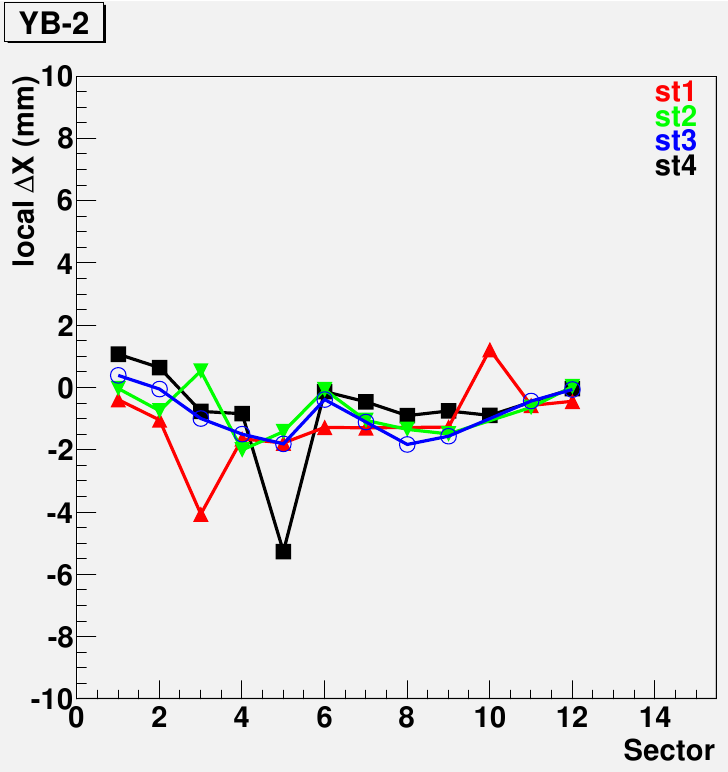
\includegraphics[width=0.25\linewidth]{hw_0T_vsPG_m2_NEW.png}

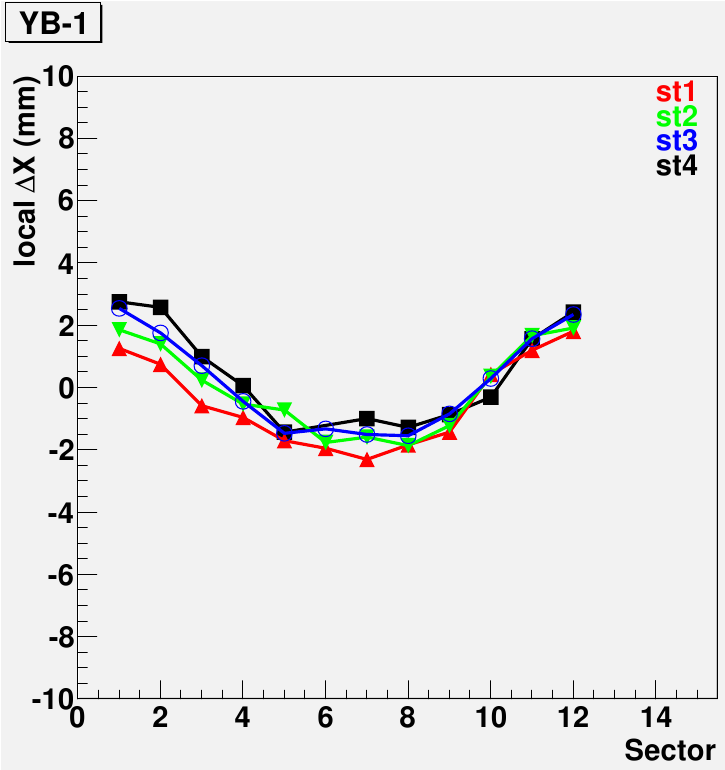
\includegraphics[width=0.25\linewidth]{hw_0T_vsPG_m1_NEW.png}
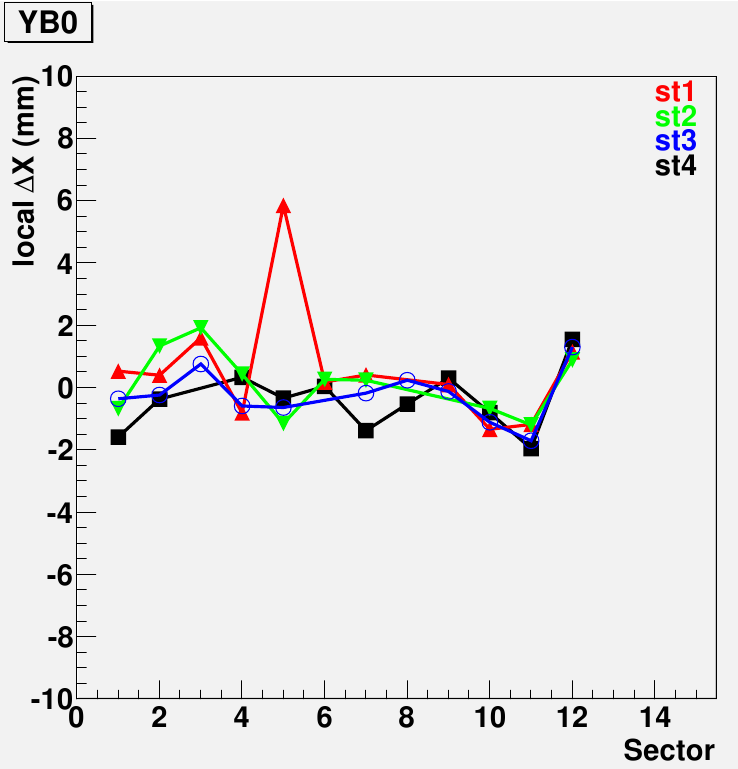
\includegraphics[width=0.25\linewidth]{hw_0T_vsPG_ze_NEW.png}
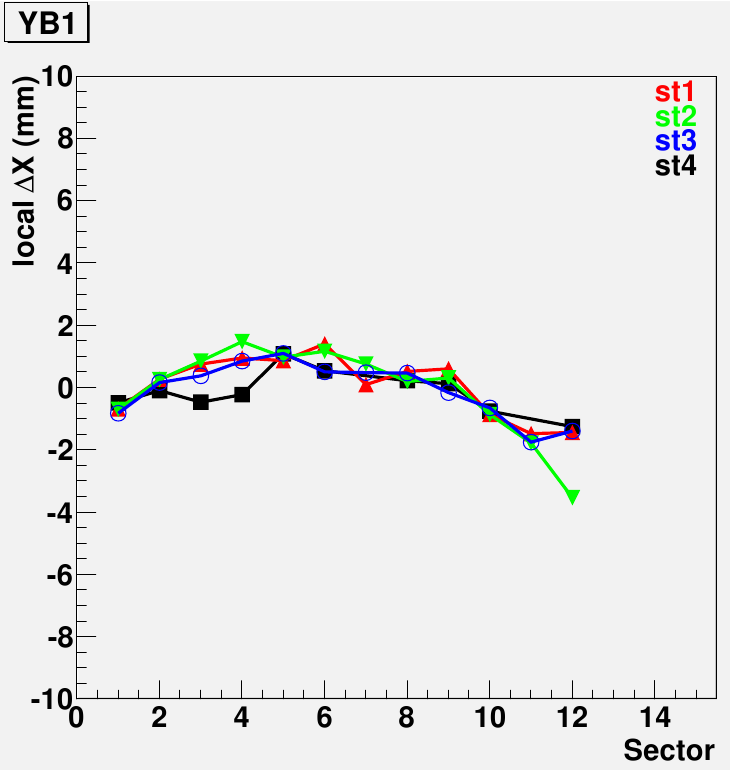
\includegraphics[width=0.25\linewidth]{hw_0T_vsPG_p1_NEW.png}
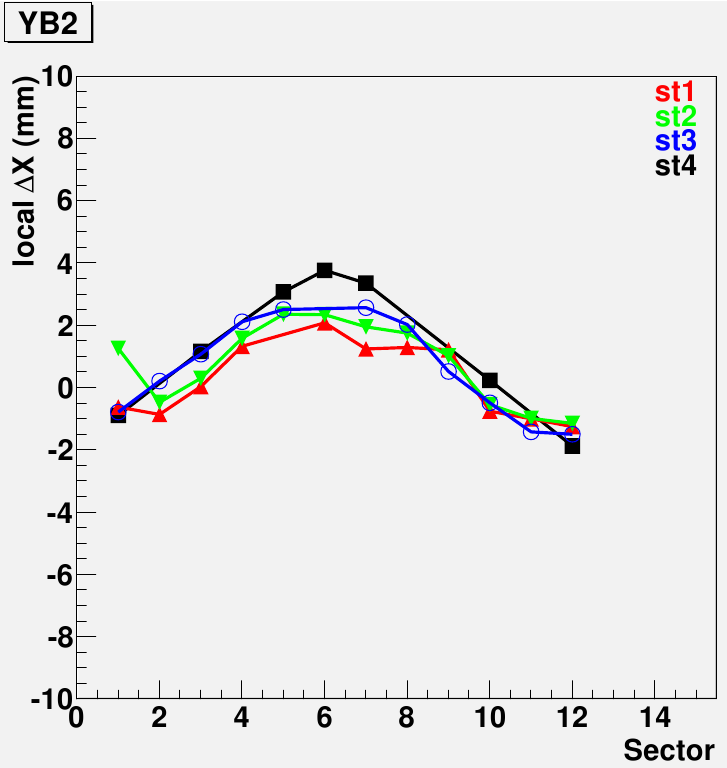
\includegraphics[width=0.25\linewidth]{hw_0T_vsPG_p2_NEW.png}
\end{frame}

\begin{frame}
\frametitle{Barrel TB and HW discrepancies}
\begin{columns}
\column{0.45\linewidth}
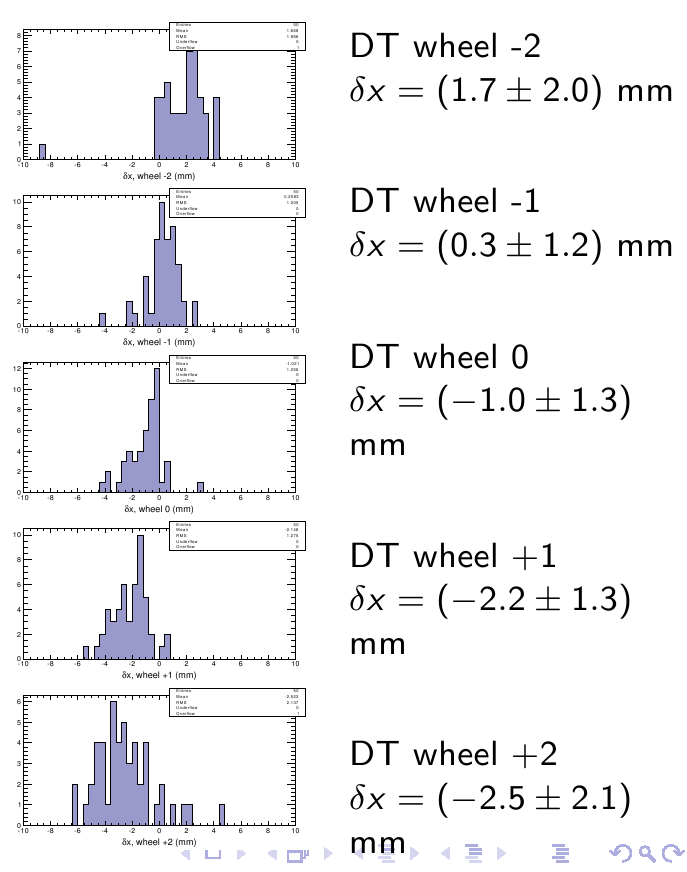
\includegraphics[width=\linewidth]{twist1.png}

\column{0.65\linewidth}
\begin{itemize}
\item Primary TB-minus-HW differences:
\begin{itemize}\setlength{\itemsep}{0.1 cm}
\item 5-chamber groups from wheel $-$2 \\ to wheel $+$2 seem to be coherently rotated: about 4~mm end-to-end
\item barrel compressed in $z$ by about 4~mm end-to-end
\item $\mathcal{O}(1.3\mbox{ mm})$ individual-chamber variations after that
\end{itemize}
\item<2> Same trends for all stations
\end{itemize}

\vfill

\only<1>{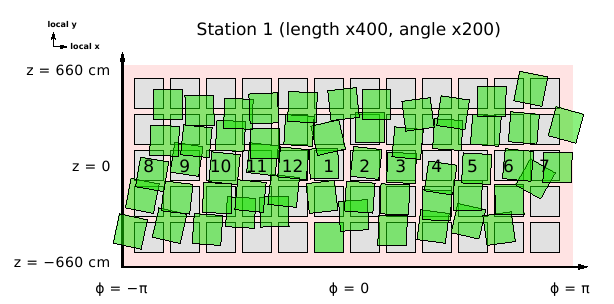
\includegraphics[width=\linewidth]{twist3_station1.png}}
\only<2>{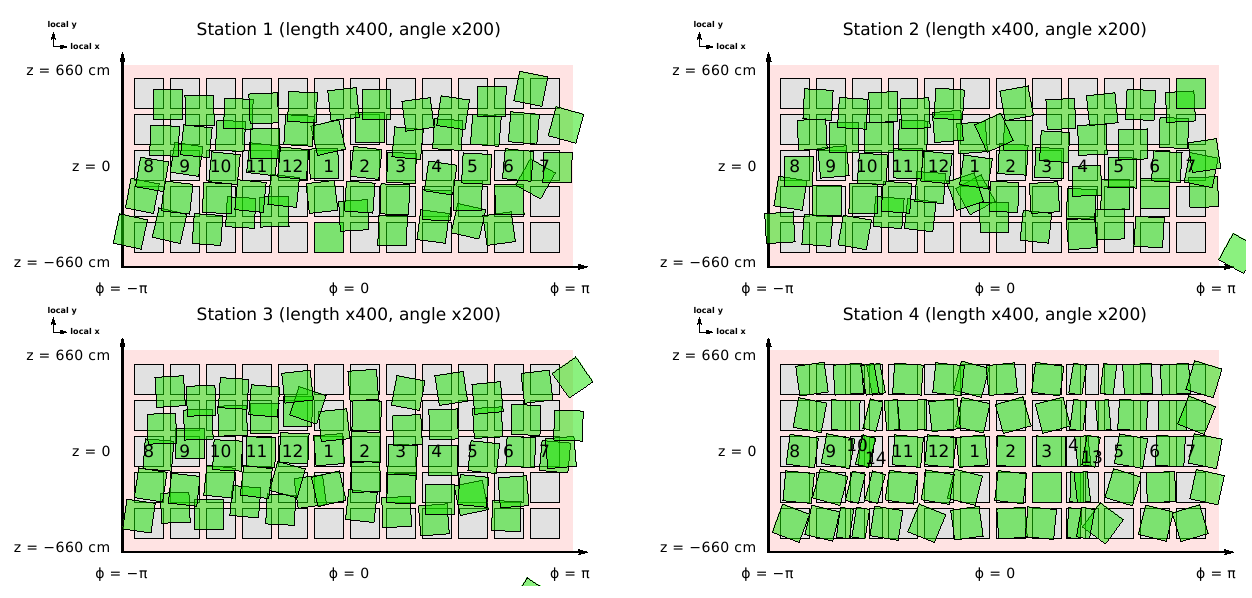
\includegraphics[width=\linewidth]{twist3.png}}
\end{columns}
\end{frame}

\begin{frame}
\frametitle{Barrel TB and HW discrepancies}
\begin{itemize}
\item Also seen at the level of residuals: these are $r\phi$ residuals
vs.\ $z$ in each 5-chamber group; dashed lines are boundaries \mbox{between chambers\hspace{-1 cm}}
\item Smooth transitions between chambers could be due to a coherent rotation in HW or a tracking bias in TB: inconclusive test
\end{itemize}
\begin{center}
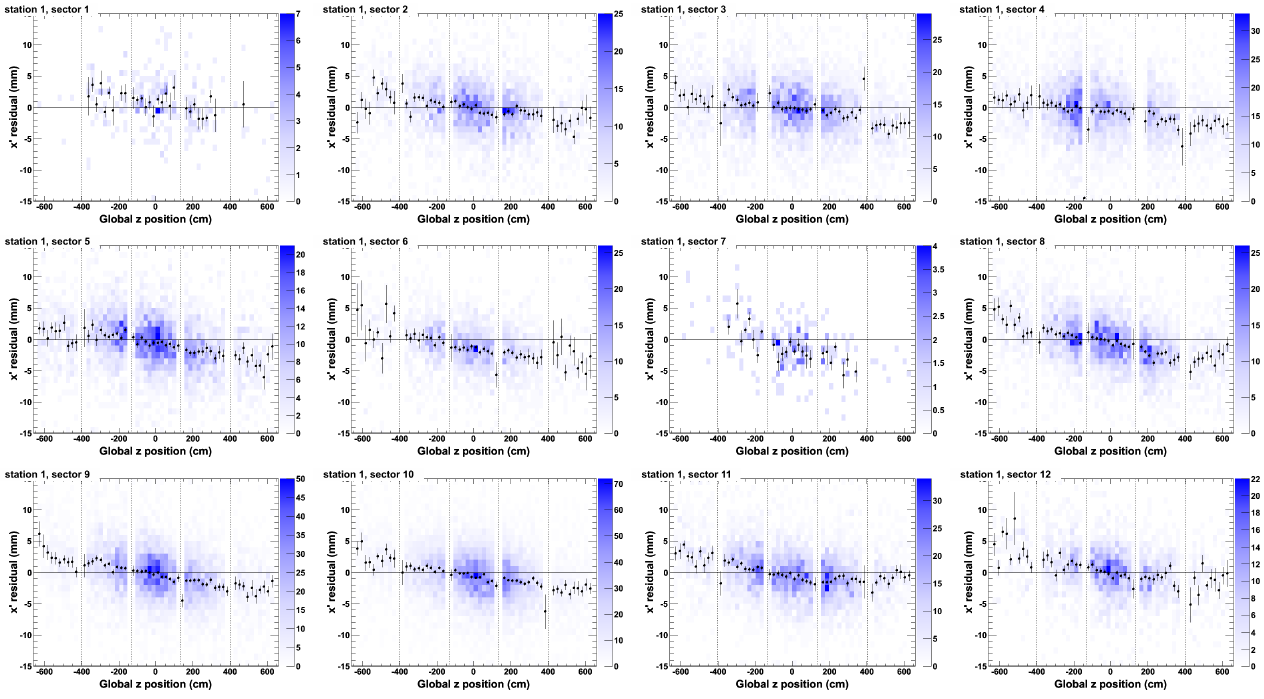
\includegraphics[width=0.9\linewidth]{twist2.png}
\end{center}

\vspace{-0.5 cm}
\mbox{\scriptsize {\bf N.B.} Vertical scales are $\pm$15~mm, horizontal scales span the barrel ($\pm$660~cm) \hspace{-1 cm}}
\end{frame}

\begin{frame}
\frametitle{Station-by-station dependence}
\begin{columns}
\column{0.5\linewidth}
\begin{itemize}
\item If the effect were due to a bias in input tracks, e.g.\ a global
distortion of the tracker leading to $z$-dependent $\Delta \phi$
errors, then its magnitude would scale with distance from the tracker

\mbox{ } \hfill 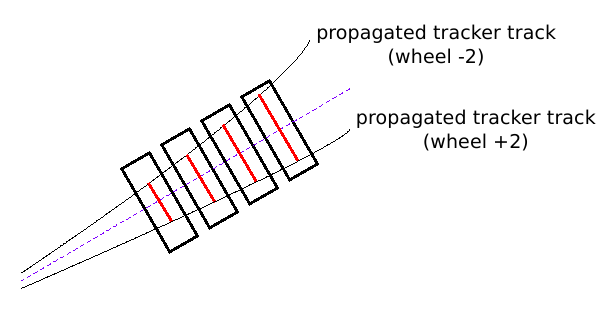
\includegraphics[width=0.75\linewidth]{growth_with_station.png} \hfill \mbox{ }

\item \textcolor{darkblue}{Test:} fit each 5-chamber group of residuals to a straight line
(50 in all) and make histograms of the resulting slopes
\item \textcolor{darkblue}{Result:} strongly peaked at the same slope
  for all four stations, though station~4 has almost twice the radius of
  station~1
\end{itemize}

\column{0.5\linewidth}
\begin{columns}
\column{0.5\linewidth}
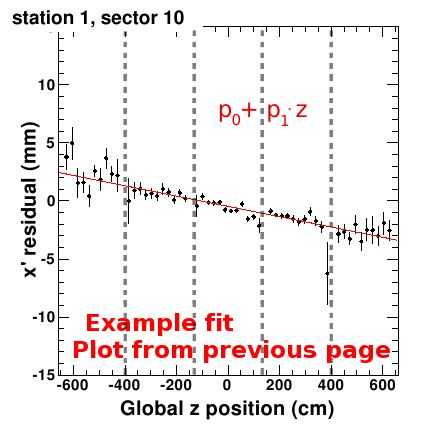
\includegraphics[width=\linewidth]{growth_with_station2.png}
\column{0.5\linewidth}
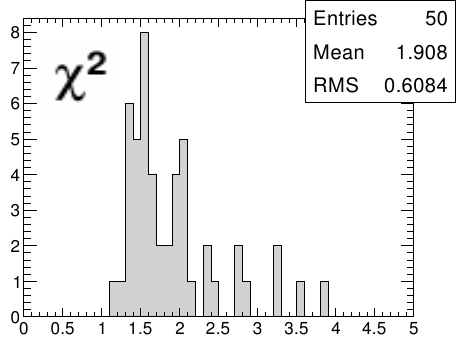
\includegraphics[width=\linewidth]{growth_with_station_chi2.png}
\end{columns}

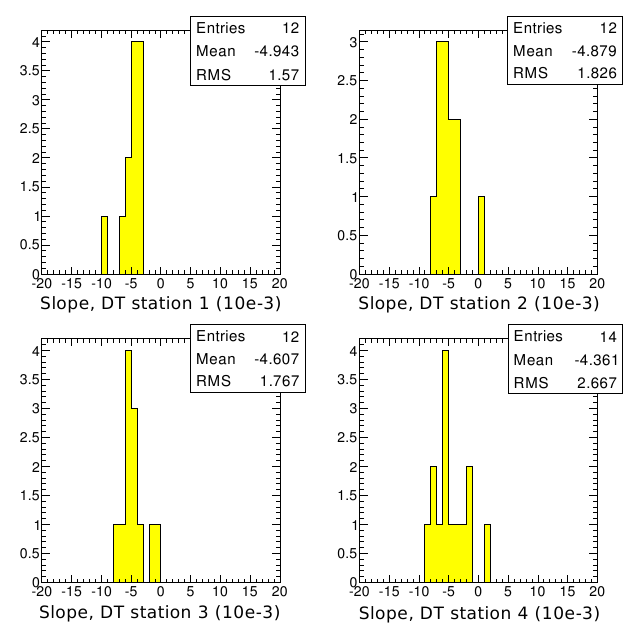
\includegraphics[width=\linewidth]{growth_with_station3.png}
\end{columns}
\end{frame}

\begin{frame}
\frametitle{Tiltmeter test}

\begin{itemize}
\item The end of each HW measurement device in the barrel (MAB) is
  equipped with a tiltmeter to sense rotation with respect to gravity
\end{itemize}

\begin{columns}
\column{0.15\linewidth}
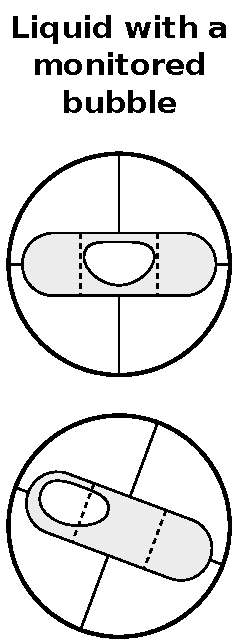
\includegraphics[width=\linewidth]{wassermeters.pdf}

\column{0.7\linewidth}
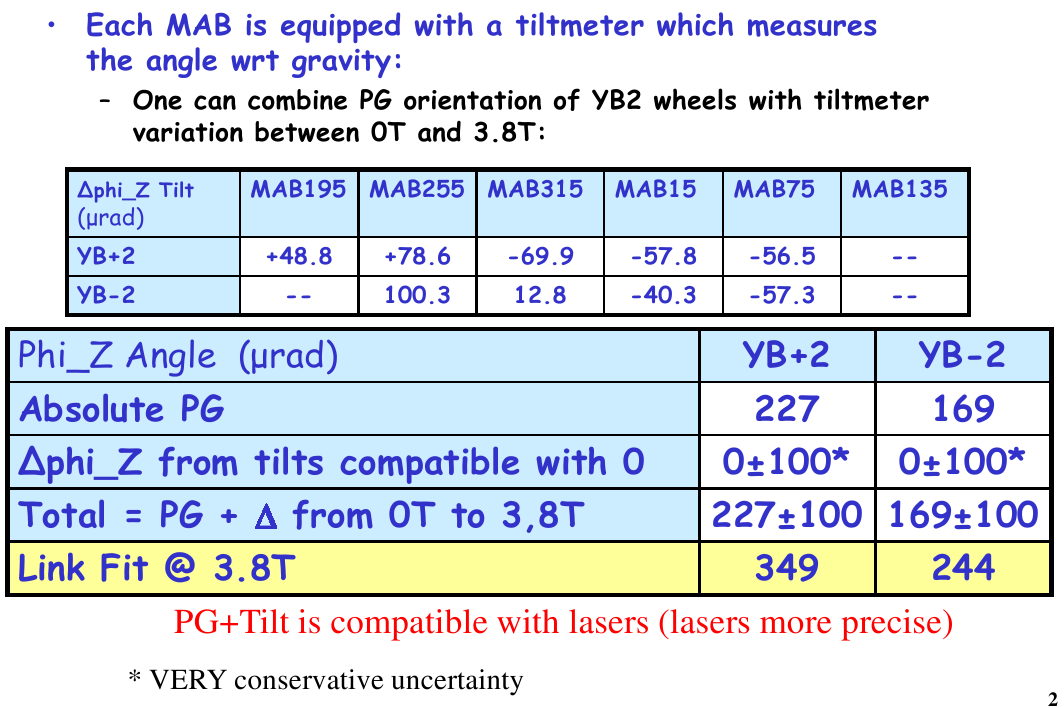
\includegraphics[width=\linewidth]{inclinometers.png}
\end{columns}

\vfill
\begin{itemize}
\item Constraint from gravity direction $+$ PG: \mbox{110 $\pm$ 140~$\mu$rad} $\to$ \mbox{0.47 $\pm$ 0.63~mm} at barrel ends, in contraction with TB's 4~mm
\item Independent of barrel HW procedure: TB is the one out of three independent measurements which differs
\end{itemize}
\end{frame}

\begin{frame}
\frametitle{Summary of DT alignment}
\begin{itemize}
\item We have two independent geometries, HW and TB, which agree in
  the major corrections with respect to design, but disagree in the details
\item Primary difference: 4~mm end-to-end rotation and scaling trends with respect to wheel (global $z$)
\begin{itemize}\setlength{\itemsep}{0.2 cm}
\item simple explanations have been ruled out, and we still have contradictory evidence among TB, HW, and the tiltmeters
\item zero-field PG-vs-HW is consistent with this picture but doesn't imply any new constraints because wheel-to-wheel PG has $\mathcal{O}(\mbox{mm})$ uncertainties
\item we don't have a proof that either TB or HW is more trustworthy, and hence will leave the geometry in the DB as it is until we sort this out
\end{itemize}
\item Proposal: unchanged HW-derived DTAlignmentRcd
\end{itemize}
\end{frame}

\begin{frame}
\frametitle{DT alignment uncertainty}
\begin{itemize}
\item We now have a handle on DT alignment systematic uncertainty: the TB-minus-HW difference
\item The known shape and magnitude of the discrepancy can be used to
  quantify systematic uncertainties in track parameters and physics observables
\item Left: track curvature error vs.\ $\eta$ with a 4~mm end-to-end twist of the barrel (tracks from $Z'$ with $m_{Z'}$ = 1100~GeV/$c^2$)
\item Right: smearing of 1100 and 2000~GeV/$c^2$ $Z'$ mass distributions with no bias (black), \textcolor{red}{z-scaling (red)}, and \textcolor{blue}{twist (blue)} (with $|\eta| < 1$)
\end{itemize}

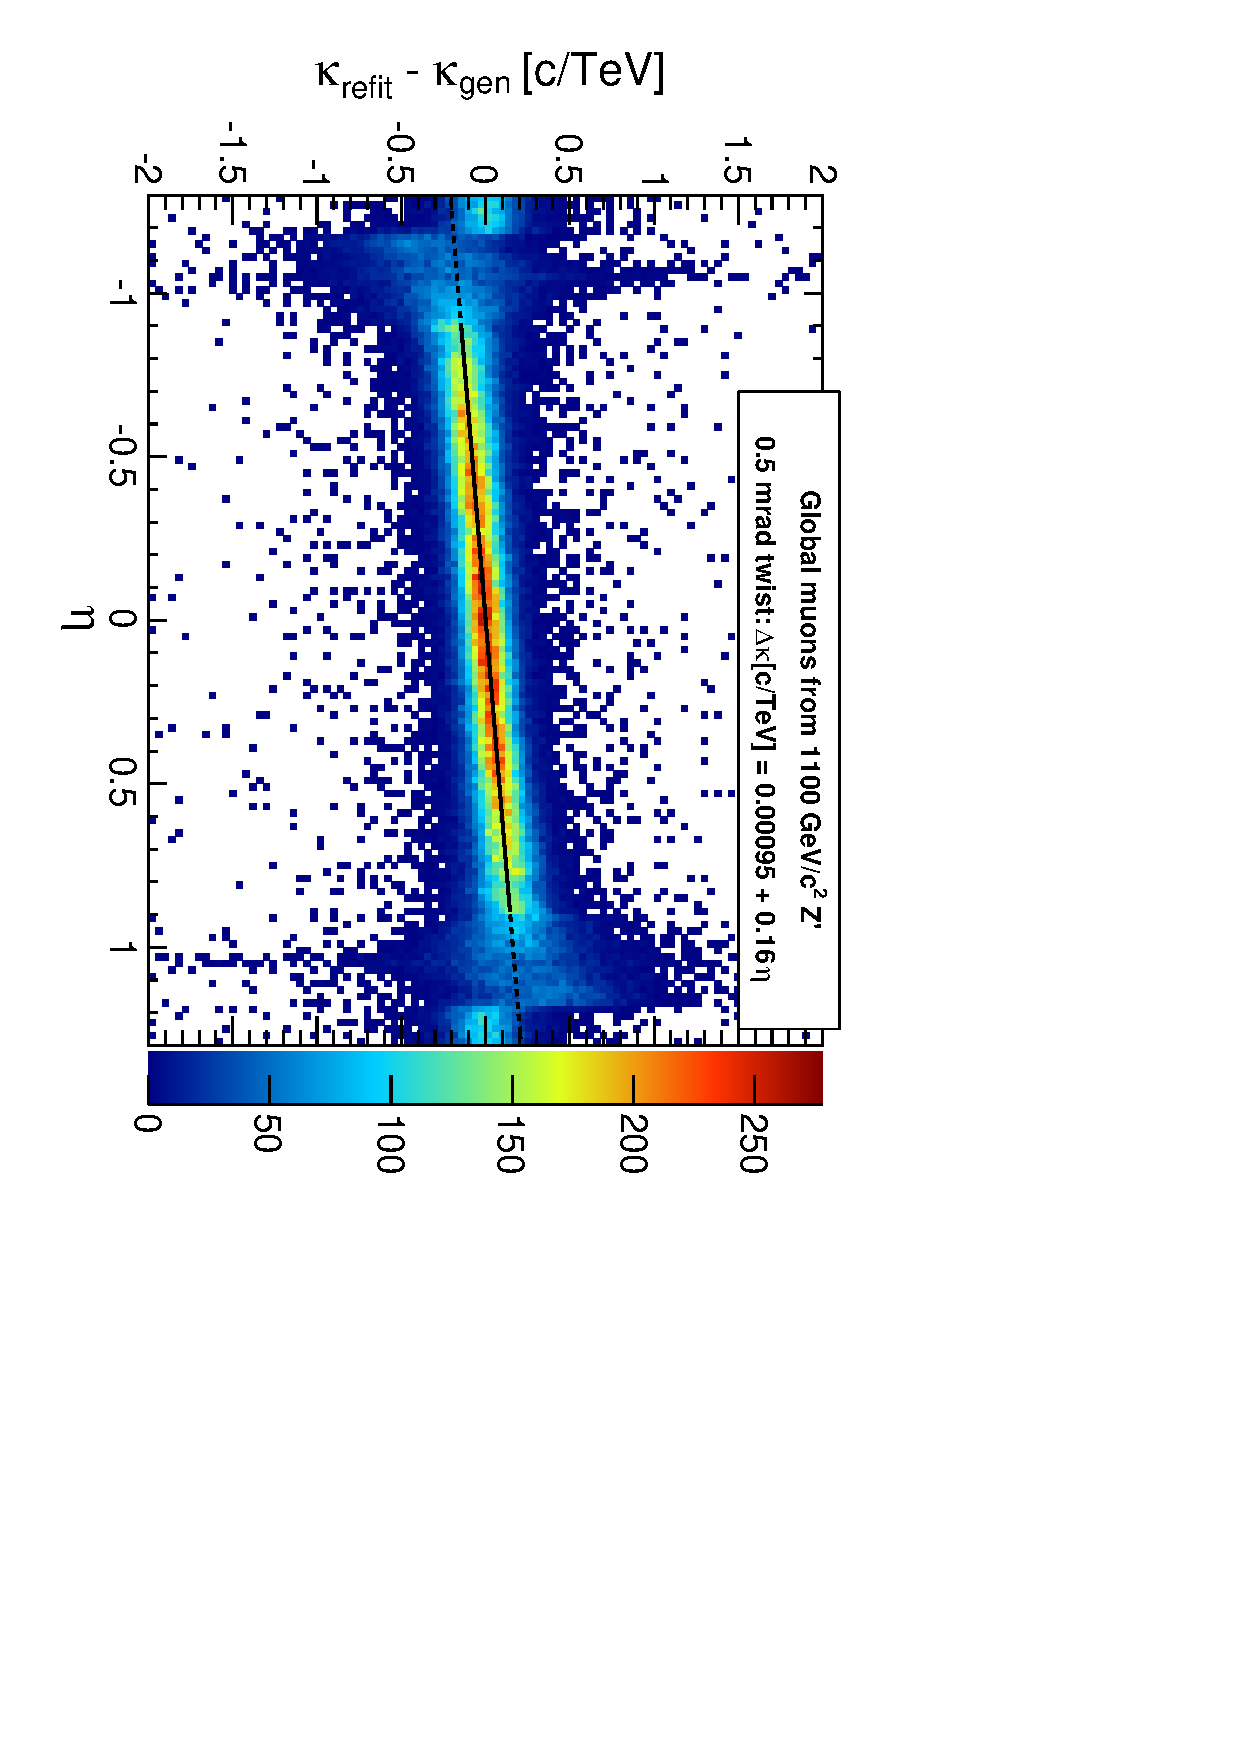
\includegraphics[width=2.5 cm, angle=90]{curvbias_vseta_twist0_5mrad_1100_GlobalMuons2.pdf}
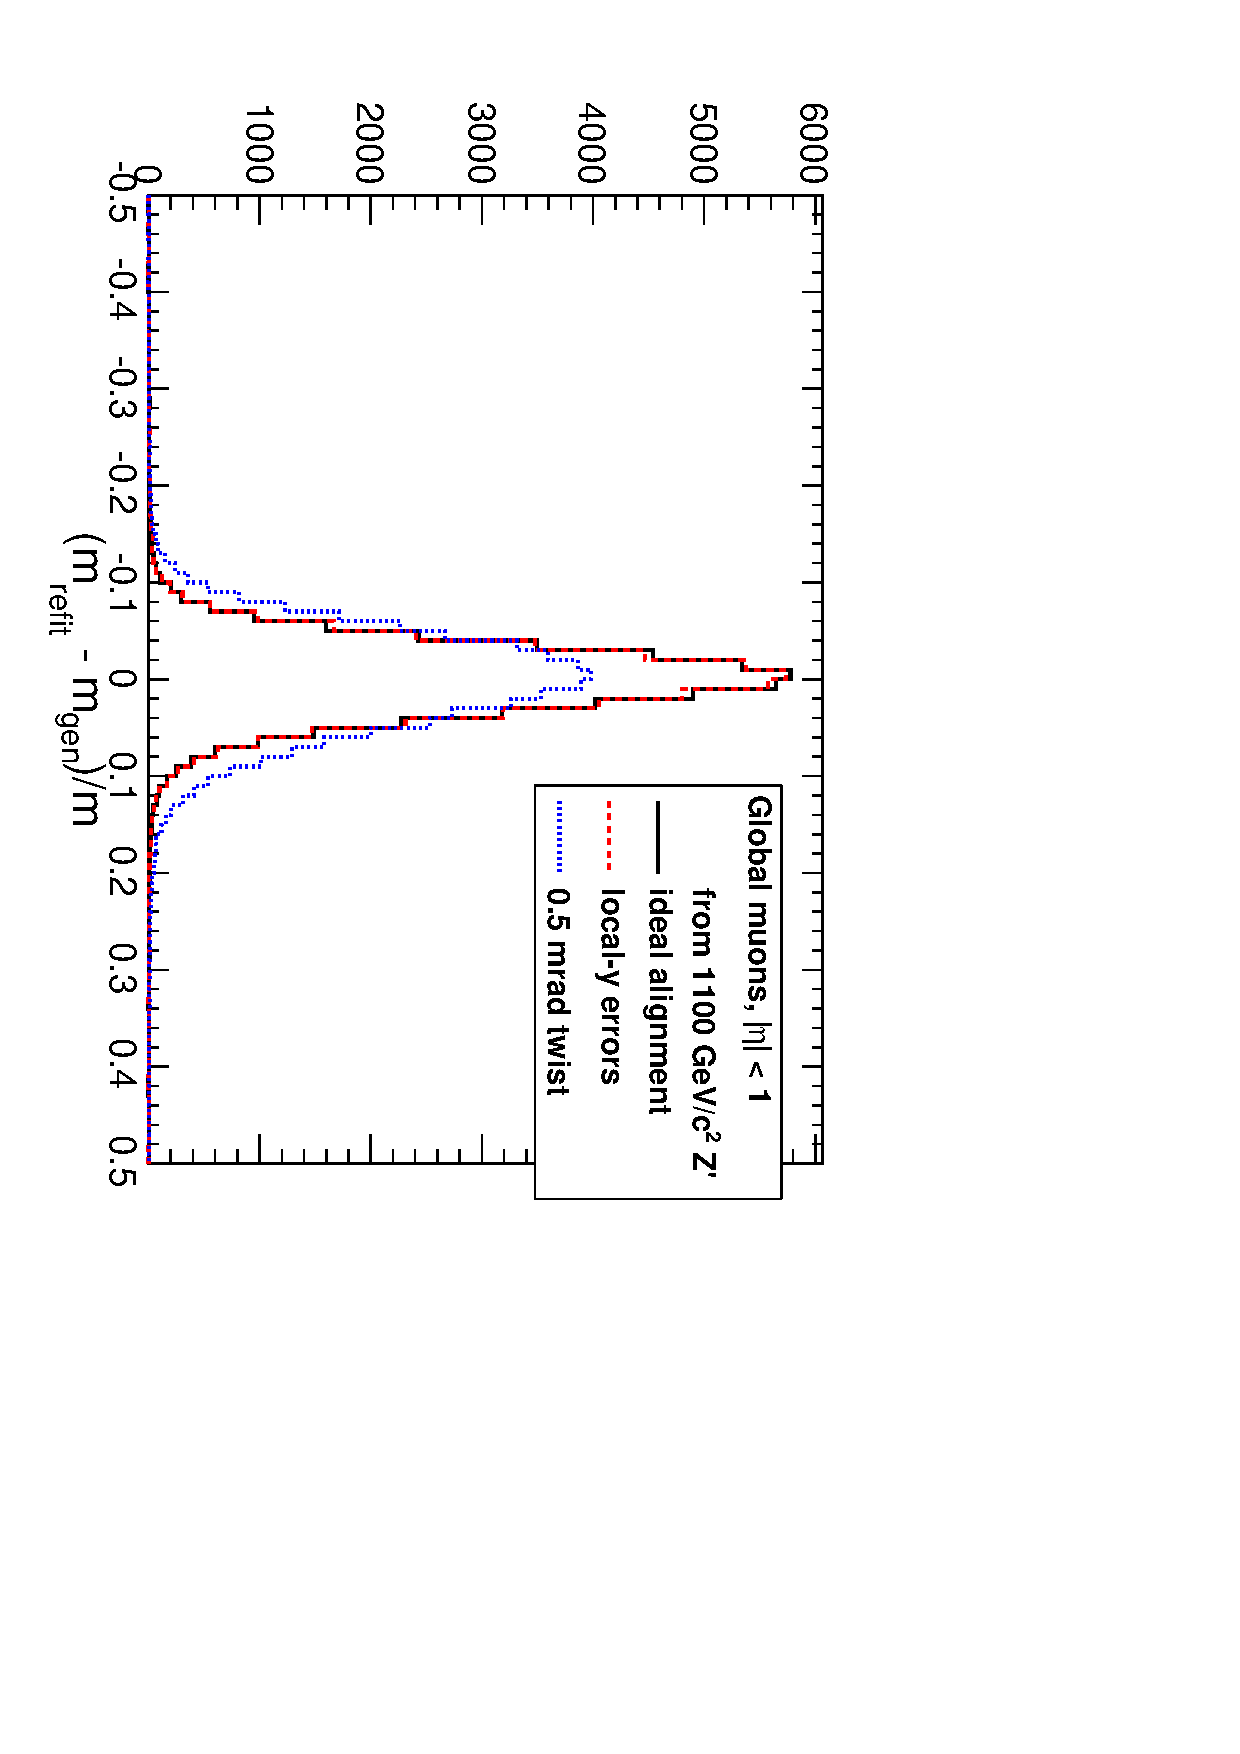
\includegraphics[width=2.5 cm, angle=90]{massdistribution_1100_GlobalMuons2.pdf}
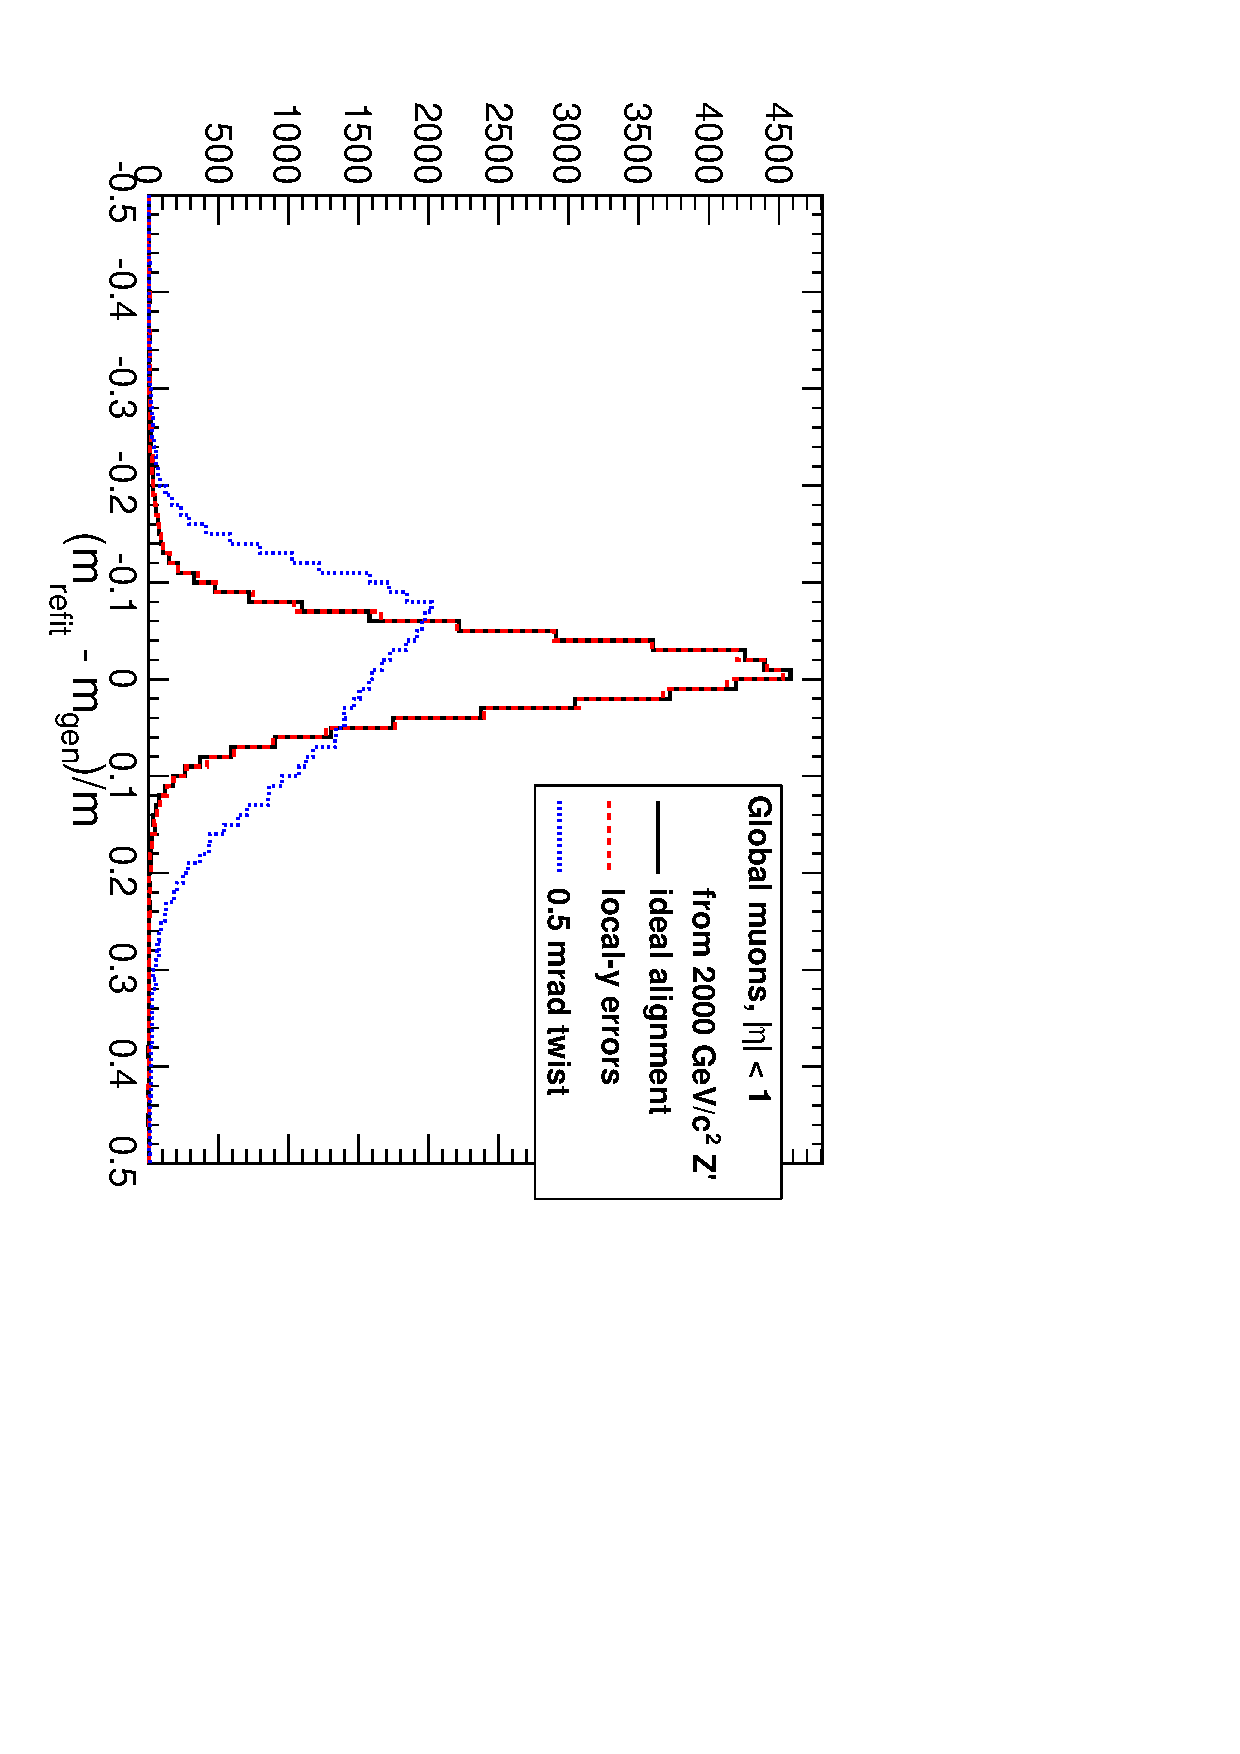
\includegraphics[width=2.5 cm, angle=90]{massdistribution_2000_GlobalMuons2.pdf}

\begin{itemize}
\item Full details belong in a different talk
\end{itemize}
\end{frame}

\begin{frame}
\frametitle{Endcap geometry}
\begin{itemize}\setlength{\itemsep}{0.25 cm}
\item Endcap has fewer points of comparison between TB and HW
\begin{itemize}
\item HW measures disk-bowing and $z$-compression toward solenoid; TB does not (with much precision)
\item TB measures $r\phi$ positions and rotations-in-transverse plane of all chambers; HW only monitors six chambers in each ring
\end{itemize}
\item Systematic HW-minus-TB comparision is in development, but
  because there are so few points of comparison, it is harder to
  distinguish measurement differences from coordinate frames

\item We do have a geometry which combines orthogonal degrees of
  freedom (next page)

\vspace{0.5 cm}
\item Currently in the database: only disk-bowing and $z$-compression
  from CRAFT-08, no information from tracks or even PG
\end{itemize}
\end{frame}

\begin{frame}
\frametitle{Combined endcap geometry}
\begin{enumerate}
\item HW provides disk-bowing and $z$-compression toward solenoid
\item Beam-halo tracks measure $r\phi$ and $\phi_z$ of chambers
  relative to their neighbors; this is used to build a complete
  geometry of each disk
\item Any missing beam-halo information is filled in by photogrammetry
  in a combined fit

\hfill 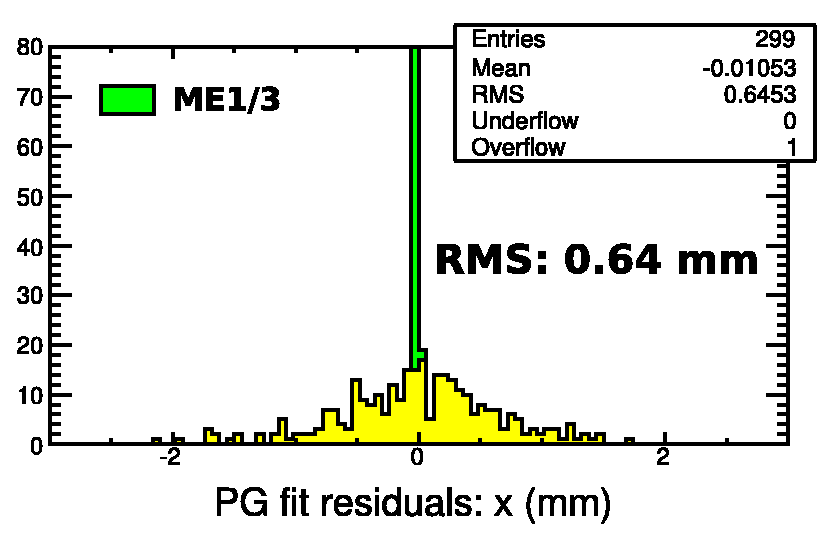
\includegraphics[width=0.4\linewidth]{beamhalo-PG.png}

\vspace{-2.8 cm}
\begin{itemize}
\item beam-halo uncertainties $\ll$ \\ photogrammetry uncertainties, \\
  except for chambers with \\ electronics issues and the shadow \\ in the
  beam-halo distribution due \\ to the LHC floor
\item photogrammetry is consistent with the combined fit at the level of 0.6~mm
\end{itemize}

\item Correct disk positions in the transverse plane (global $x$, $y$,
  $\phi_z$) with cosmic ray tracks from the tracker (using new GlobalPositionRcd)
\end{enumerate}
\end{frame}

%% \begin{frame}
%% \frametitle{Outline}
%% \begin{itemize}\setlength{\itemsep}{0.75 cm}
%% \item 
%% \end{itemize}
%% %% \hspace{-0.83 cm} \textcolor{darkblue}{\Large Outline2}
%% \end{frame}

%% \section*{First section}
%% \begin{frame}
%% \begin{center}
%% \Huge \textcolor{blue}{First section}
%% \end{center}
%% \end{frame}

\begin{frame}
\frametitle{Locations of new constants}
\begin{itemize}\setlength{\itemsep}{1 cm}
\item Updated GlobalPositionRcd: {\tiny /afs/cern.ch/user/s/spiridon/public/JUN6\_MuBarrelHW\_Tracker\_ichep10\_GlobalPositionRcd.db}

\item DT HW alignment: offline DB tag ``DTAlignment\_2009\_v4\_offline''
\item Updated CSC combined alignment:

{\tt \scriptsize /afs/cern.ch/user/p/pivarski/public/JUN5\_CSC\_beamhalo-PG-diskXYphiZ.db}

(note: still waiting on final disk-$z$ corrections to CSC geometry or will fall-back to a default set)

\end{itemize}
\end{frame}

\begin{frame}
\frametitle{Conclusions}
\begin{itemize}\setlength{\itemsep}{0.5 cm}
\item Significant improvements to the muon geometry currently in the
  database are available
\item Comparisons between track-based and hardware alignments in the
  barrel are not in sufficient agreement, but the discrepancies are
  systematic, suggesting a single surmountable problem
\item With two independent measurements of the barrel alignment, we
  can quantify alignment systematic uncertainties in a way that can be
  propagated to analyses
\item TB-minus-HW comparisons are more difficult in the endcap, but
  TB-minus-PG is precise
\end{itemize}
\label{numpages}
\end{frame}

\end{document}
